\chapter{Resultados experimentales}

    \section{Comunicación RS232}

    Una vez implementado el generador de semillas y el mapa caótico es necesario poder transmitir la información para su posterior análisis. Para esto se realizó la implementación de una comunicación RS232 con un baudrate a 15200 sin bit de paridad. Como solo es necesario transmitir datos del sistema a una computadora  solo se implementó la transmisión. En la Figura \ref{fig:C1_architecture_rs232} se muestra el diagrama a bloques de la transmisión y en la Figura \ref{fig:C0_fsm_rs232} el diagrama de la maquina de estados que controla la transmisión.

        \begin{figure}[hbtp]
            \caption{Diagrama de bloques de transmisión RS232.}
            \centering
            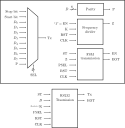
\includegraphics[width=0.6\linewidth]{C1_architecture_rs232}
            \label{fig:C1_architecture_rs232}
        \end{figure}

        Se eligió no transmitir el bit de paridad para que los paquetes enviados sean fáciles de procesar, además esto aumenta un poco la velocidad de transmisión ya que se manda un bit menos, y para nuestro caso, en el que se requieren transmitir 100 millones de bits aleatorios es un ahorro significativo. 

        \begin{figure}[hbtp]
            \caption{Máquina de estados para la transmisión RS232.}
            \centering
            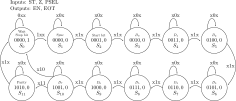
\includegraphics[width=0.8\linewidth]{C0_fsm_rs232}
            \label{fig:C0_fsm_rs232}
        \end{figure}	

    \section{TRNG híbrido}

        De manera que el sistema completo se muestra en la Figura \ref{fig:D0_system}. Este consiste en el generador de semillas aleatorios utilizando el ERO-TRNG como núcleo, el mapa caótico el cual calcula cada dos ciclos de reloj una iteración nueva, la operación mod 256 para extraer 16 bits aleatorios del mapa, la comunicación RS232 en conjunto un multiplexor para mandar paquetes de 8 bits y una maquina de estados cuyo diagrama se muestra en la Figura \ref{fig:D1_fsm_system}, que controla y sincroniza todo el sistema.

         \begin{figure}[hbtp]
            \caption{Diagrama de bloques de TRNG híbrido.}
            \centering
            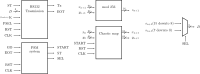
\includegraphics[width=0.9\linewidth]{D0_system}
            \label{fig:D0_system}
        \end{figure}

        El generador funciona de la siguiente manera. Cuando el sistema se enciende el generador de semillas comienza a generar bits aleatorios utilizando el ERO-TRNG interno, cuando este proceso termina la señal READY se activa avisando que hay una semilla valida en SEED y este proceso no vuelve a ocurrir a menos que la FPGA se reinicie.

       El sistema espera que el usuario active la señal BUTTON para comenzar. Cuando el sistema se activa la maquina de estados calcula una iteración del mapa caótico, posteriormente se activa la transmisión que envía los primeros 8 bits aleatorios por medio del protocolo de comunicación RS232, una vez concluida, se envían los siguiente 8 bits aleatorios y el sistema regresa a esperar por la señal BUTTON. 

       Si la señal BUTTON se queda activa este proceso se vuelve cíclico y se generan tantos bits aleatorios cómo el usuario desee.

       \begin{figure}[hbtp]
            \caption{Máquina de estados de TRNG híbrido.}
            \centering
            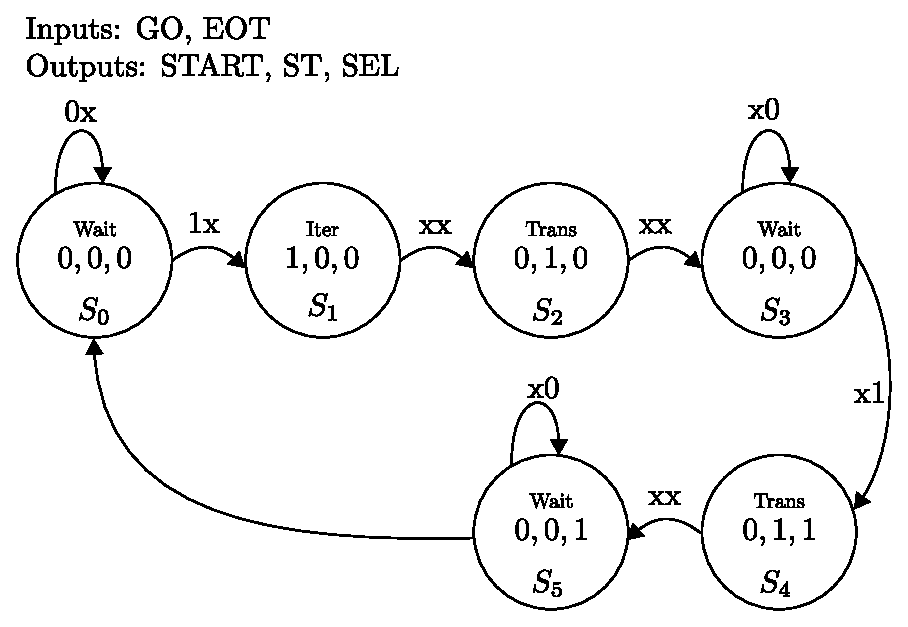
\includegraphics[width=0.7\linewidth]{D1_fsm_system}
            \label{fig:D1_fsm_system}
        \end{figure}

        \section{Pruebas estadísticas}

        Utilizando una computadora con Windows 10 y el programa PuTTY como interfaz, el sistema corriendo se ejecutó por aproximadamente 20 minutos y se almacenaron alrededor 100 millones de bits aleatorios, lo que representan un archivo de aproximadamente 700,000 KB. Los datos se almacenaron como caracteres ASCII donde cada carácter contiene 8 bits aleatorios. Utilizando un programa de C se convirtieron los caracteres a números binarios para poder ingresarse con facilidad a la suite de pruebas estadísticas NIST \cite{Nist2010,Turan2018}. En la Tabla \ref{tab:resultados_NIST_100} se muestran los resultados de las pruebas estadísticas NIST del sistema a 100 millones de bits aleatorios y en la Tabla \ref{tab:resultados_NIST_1000} se muestran los resultados de las pruebas estadísticas NIST del sistema a 1000 millones de bits aleatorio.

\begin{table}[htbp]
  \centering
  %\resizebox{\linewidth}{!}{ 
  \caption{Resultados de la aplicación de las pruebas NIST al TRNG híbrido implementado en aritmética de punto fijo con 100 millones de datos.}
    \begin{NiceTabular}{|l|c|c|}
    \CodeBefore
    \rowcolor{lightgray}{1}
    \Body
    \hline
    Test name                 & p-value  & \%   \\
    \hline
    Frequency                 & 0.383827 & 0.99 \\
    \hline
    Block frequency           & 0.108791 & 1.00 \\
    \hline
    Cumulative sums           & 0.401199 & 1.00 \\
    \hline
    Runs                      & 0.971699 & 0.99 \\
    \hline
    Longest Run               & 0.759756 & 1.00 \\
    \hline
    Rank                      & 0.383827 & 0.99 \\
    \hline
    FFT                       & 0.383827 & 0.99 \\
    \hline
    NonOverlapping template   & 0.480298 & 0.99 \\
    \hline
    Overlapping template      & 0.883171 & 0.99 \\
    \hline
    Universal                 & 0.574903 & 0.99 \\
    \hline
    Approximate entropy       & 0.759756 & 0.98 \\
    \hline
    Random excursions         & 0.265539 & 0.99 \\
    \hline
    Random excursions variant & 0.312463 & 0.99 \\
    \hline
    Serial                    & 0.595604 & 1.00 \\
    \hline
    Linear complexity         & 0.574903 & 1.00 \\
    \hline
    \end{NiceTabular}%
    %}
  \label{tab:resultados_NIST_100}%
\end{table}%
    
\begin{table}[htbp]
  \centering
  %\resizebox{\linewidth}{!}{ 
  \caption{Resultados de la aplicación de las pruebas NIST al TRNG híbrido implementado en aritmética de punto fijo con 1000 millones de datos.}
    \begin{NiceTabular}{|l|c|c|}
    \CodeBefore
    \rowcolor{lightgray}{1}
    \Body
    \hline
    Test name                 & p-value  & \%   \\
    \hline
    Frequency                 & 0.587274 & 0.989 \\
    \hline
    Block frequency           & 0.796268 & 0.998 \\
    \hline
    Cumulative sums           & 0.848047 & 0.990 \\
    \hline
    Runs                      & 0.614226 & 0.988 \\
    \hline
    Longest Run               & 0.660012 & 0.992 \\
    \hline
    Rank                      & 0.255705 & 0.990 \\
    \hline
    FFT                       & 0.072514 & 0.994 \\
    \hline
    NonOverlapping template   & 0.481082 & 0.989 \\
    \hline
    Overlapping template      & 0.143686 & 0.988 \\
    \hline
    Universal                 & 0.228367 & 0.988 \\
    \hline
    Approximate entropy       & 0.786830 & 0.992 \\
    \hline
    Random excursions         & 0.447308 & 0.990 \\
    \hline
    Random excursions variant & 0.405096 & 0.992 \\
    \hline
    Serial                    & 0.124135 & 0.993  \\
    \hline
    Linear complexity         & 0.008816 & 0.989 \\
    \hline
    \end{NiceTabular}%
    %}
  \label{tab:resultados_NIST_1000}%
\end{table}%
        
    La proporción mínima de aprobados para cada prueba estadística es aproximadamente de 96 para 100 millones de secuencias binarias y de 980 para 1000 millones de secuencias binarias. Para ambos casos todas las pruebas pasaron la proporción mínima. 

    Además analizando la distribución de probabilidad de unos y ceros que se muestra en la Figura \ref{fig:J3_distribucion} es consistente con el análisis en simulación y el histograma, que se muestra en la Figura \ref{fig:J4_distribucion} esta perfectamente distribuido de manera uniforme, por lo que de manera cualitativa y cualitativa este TRNG híbrido cumple con las requisitos estadísticos.
 

        \begin{figure}[hbtp]
            \caption{Distribución de 100 millones de palabras de 16 bits experimentales.}
            \centering
            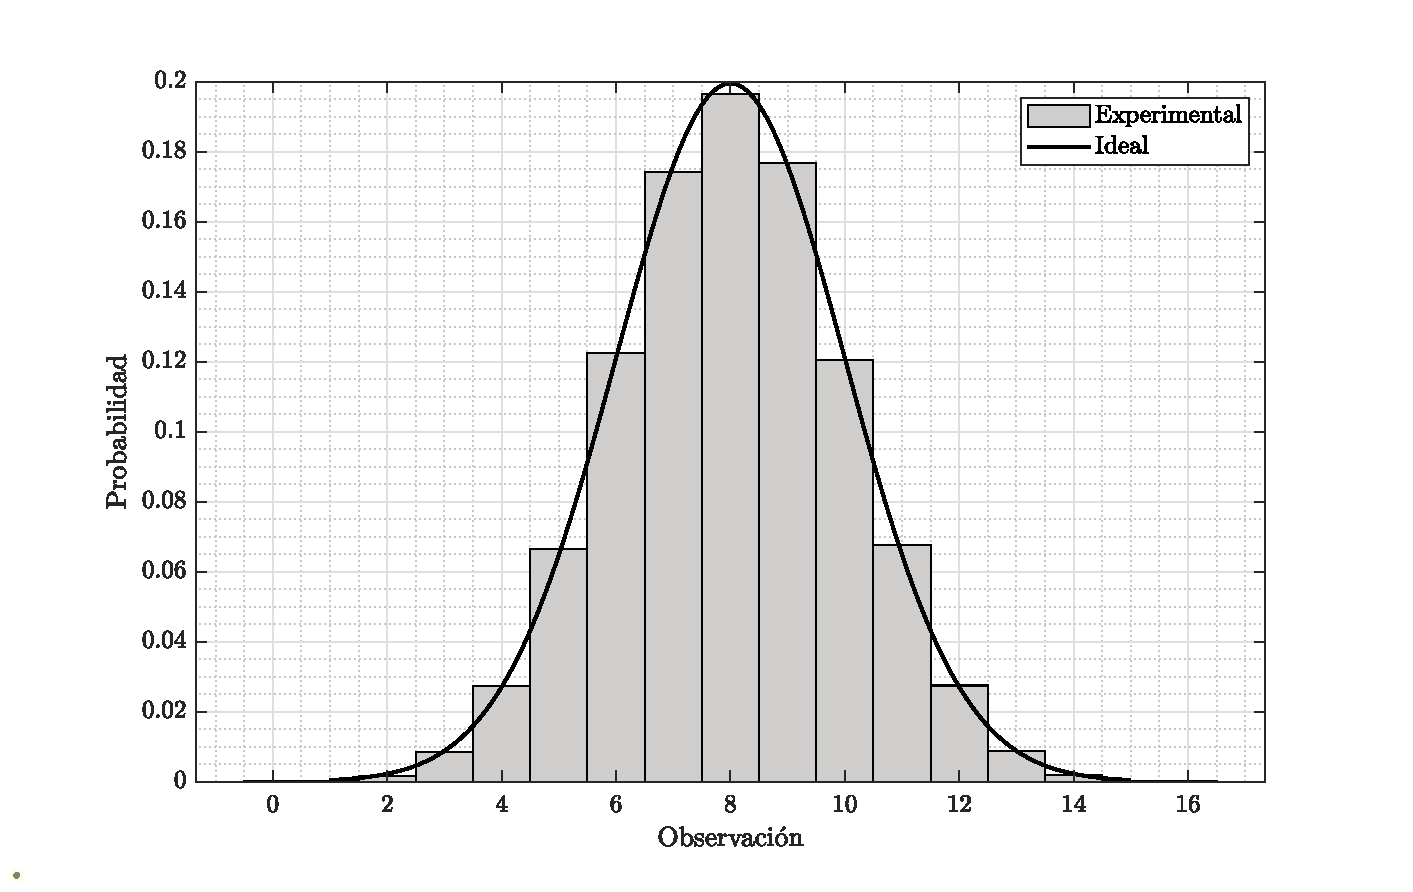
\includegraphics[width=0.8\linewidth]{J3_distribucion}
            \label{fig:J3_distribucion}
        \end{figure}


        \begin{figure}[hbtp]
            \caption{Histograma de resultados experimentales primeros 100 mil secuencias binarias.}
            \centering
            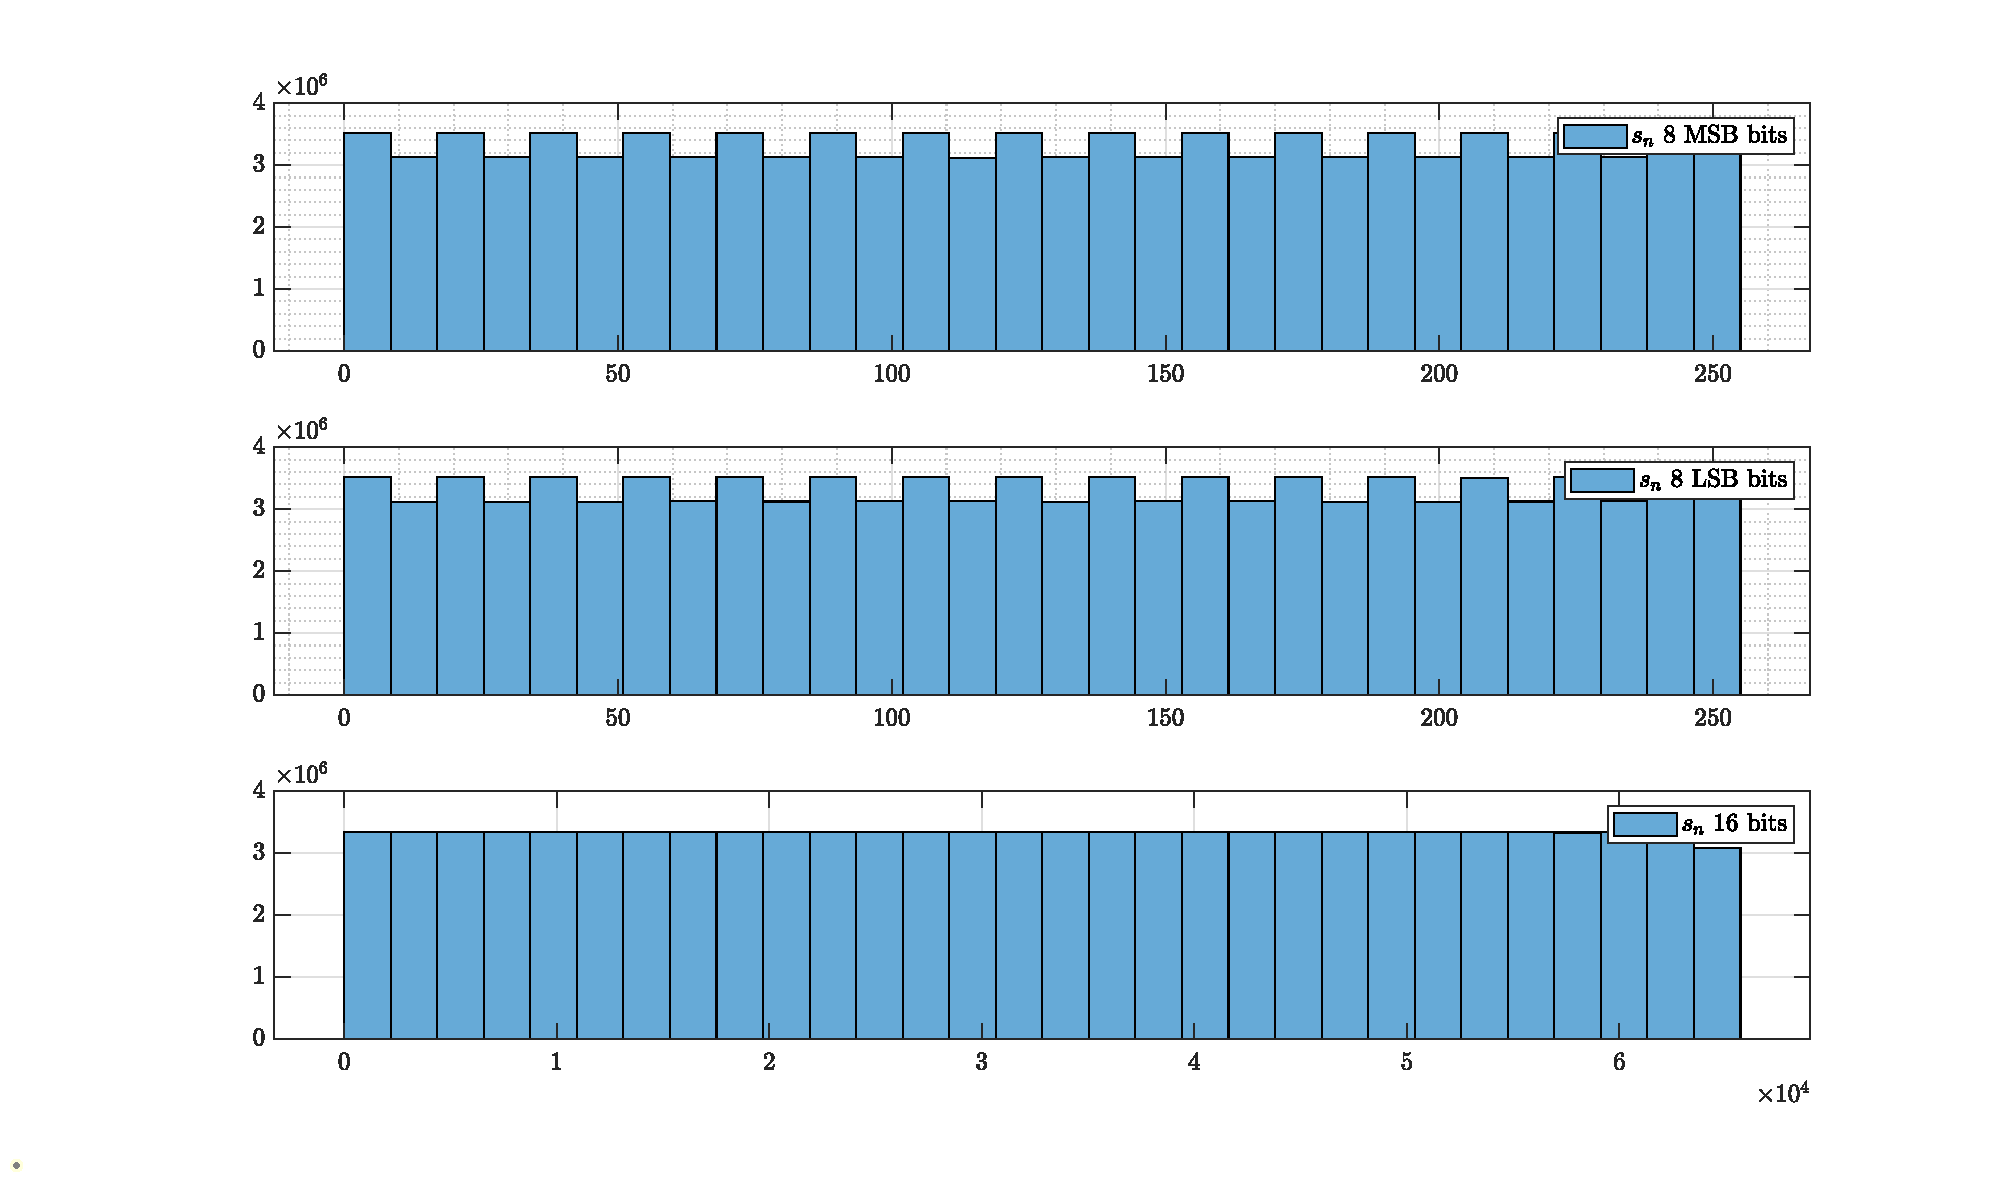
\includegraphics[width=0.9\linewidth]{J4_distribucion}
            \label{fig:J4_distribucion}
        \end{figure}



    \section{Uso de recursos y velocidad}

        En cuanto recursos utilizados, en este trabajo se utilizó la tarjeta de desarrollo Basys 3 del fabricante Digilent, la cual cuenta con un FPGA Artix 7 xc7a35tcpg236-1 y un oscilador de 100 MHz. Esta tarjeta se encuentra dentro de la gama media-baja en lo concerniente a recursos, ya que dispone de una cuarta parte o incluso menos de los recursos de tarjetas hermanas como la Nexys A7 o la Zybo Z7. En la Tabla \ref{tab:recursos} se muestran los recursos utilizados todos los multiplicadores son multiplicadores completos. Debido que el sistema necesita 11 multiplicadores de 64 bits, y un solo multiplicador de este tamaño utiliza aproximadamente un 18 \% de los DSP disponibles, el diseño casi utiliza la totalidad de la FPGA. 

        \begin{table}[htbp]
            \centering
            \caption{Uso de recursos del TRNG híbrido con multiplicadores completos.}
            \begin{tabular}{|l|l|l|l|}
                \hline
                \rowcolor{lightgray} Recursos  & Utilización & Disponibles & Utilización \% \\
                \hline
                LUTs      & 17767  & 20800    & 85.42  \\
                \hline
                FF     &  148 & 41600   & 0.36 \\
                \hline
                DSP       & 90  & 90   & 100.0 \\
                \hline
            \end{tabular}
            \label{tab:recursos}
        \end{table}

        No obstante si se utilizan multiplicadores de una sola constante para todos los parámetros $a_{n}$ el uso de recursos se reduce drásticamente como se muestra en la Figura \ref{tab:recursos_op}.

        \begin{table}[htbp]
            \centering
            \caption{Uso de recursos del TRNG híbrido con multiplicadores de una sola constante en parámetros $a_{n}$.}
            \begin{tabular}{|l|l|l|l|}
                \hline
                \rowcolor{lightgray} Recursos  & Utilización & Disponibles & Utilización \% \\
                \hline
                LUTs      & 1469  & 20800    & 7.06  \\
                \hline
                FF     & 146  & 41600   & 0.35  \\
                \hline
                DSP       & 80  & 90   & 88.89  \\
                \hline
            \end{tabular}
            \label{tab:recursos_op}
        \end{table}

        Para este diseño en particular es necesario utilizar los multiplicadores de una sola constante para tener disponibles suficientes recursos para realizar otras aplicaciones en conjunto con el TRNG híbrido.

        Debido a que el sistema trabaja a una velocidad de 100 MHz y cada iteración del mapa caótico necesita 2 ciclos de reloj para calcular la iteración y un ciclo para mandar el resultado a un registro de salida, la velocidad del generador es de 30 ns y como se generan 16 bits aleatorios en ese tiempo, la velocidad de salida o throughput en inglés es de 533.33 Mbits/s, que en comparación con \cite{Fraga2021} que realizó una implementación similar en un microcontrolador de alto rendimiento de la familia STM32, en el que se alcanzó una velocidad de salida de 173.35 Kbits/s, nuestro sistema puede utilizarse para aplicaciones que requieran mayor velocidad.


